\documentclass{beamer}
%
% Full manual: http://mirror.unl.edu/ctan/macros/latex/contrib/beamer/doc/beameruserguide.pdf
%
% For more themes, color themes and font themes, see:
% http://deic.uab.es/~iblanes/beamer_gallery/index_by_theme.html
%
% Go here for all the themes: http://www.hartwork.org/beamer-theme-matrix/
% For a cheatsheet: http://www.cpt.univ-mrs.fr/~masson/latex/Beamer-appearance-cheat-sheet.pdf

%\usepackage{tikz} You can use this package to insert watermarks or draw shapes and stuff like you can do with powerpoint


\mode<presentation>
{
  \definecolor{berkeleyblue}{HTML}{003262}
  \definecolor{berkeleygold}{HTML}{FDB515}
  \usetheme{Boadilla}      % or try Darmstadt, Madrid, Warsaw, ...
  %\usecolortheme{dove} % or try albatross, beaver, crane, ...
  \setbeamercolor{structure}{fg=berkeleyblue,bg=berkeleygold}
  \setbeamercolor{palette primary}{fg=berkeleyblue,bg=berkeleygold} % changed this
  \setbeamercolor{palette secondary}{bg=berkeleyblue,fg=white} % changed this
  \setbeamercolor{palette tertiary}{bg=berkeleyblue,fg=white} % changed this
  \usefonttheme{structurebold}  % or try serif, structurebold, ...
  \useinnertheme{circles}
  \setbeamertemplate{navigation symbols}{}
  \setbeamertemplate{caption}[numbered]
  \usebackgroundtemplate{
  %\tikz[overlay,remember picture] Can insert a Berkeley watermark
  %\node[opacity=1, at=(current page.south west),anchor=south west, inner sep=2pt] {
   % 
\includegraphics[height=.5in,width=.5in]{ucseal_540_139.eps}};
}
} 

\usepackage{hyperref}

\title{\LaTeX{} Intro and Overview}
\author{Rachel Slaybaugh}
\institute{derived from Laurence Lewis}
\date{3/09/2015}

\begin{document}

\bibliographystyle{plain}

\begin{frame}
  \titlepage
\end{frame}

% Uncomment these lines for an automatically generated outline.
%\begin{frame}{Outline}
%  \tableofcontents
%\end{frame}

 %----------------------------------------------------- 
\begin{frame}{An Overview of \LaTeX{}}
	\begin{enumerate}
    	\item What \LaTeX{} is and how to get it
        \item Making documents
        \item Making presentations using \texttt{Beamer}
        \item Making posters using \texttt{Beamerposter}
        \item Rapid document/presentation prep (Markdown + \LaTeX{})
     \end{enumerate}
     \vfill
     A \LaTeX{} cheat sheet is available here:      \href{http://www.stdout.org/~winston/latex/latexsheet.pdf}{http://www.stdout.org/~winston/latex/latexsheet.pdf}
\end{frame}

 %----------------------------------------------------- 
\begin{frame}{\LaTeX{} is a typesetting language}

	\begin{itemize} % You can also use   (\setbeamercovered{transparent=30}) to set transparency
  	\item It lets you \textcolor{red}{seamlessly} transition between words and math: 
  	$$\sum_{n=0}^\infty\frac{x^n}{n!}=e^x$$
  	\item You can typeset \textcolor{red}{publication-quality} articles, books, theses, presentations, and posters
  	\item It \textcolor{red}{automatically} handles bibliographies, citations, and references for equations, images, and tables 
  	\item The easy part is learning how to type math, the hard part is the formatting
  		\begin{itemize}
    		\item But luckily, there is a \textbf{huge} user-base with lots of examples
    	\end{itemize}
	\end{itemize}
    
\end{frame}
 
 %-----------------------------------------------------   
\begin{frame}{\LaTeX{} can be used at home or online}

	\begin{itemize}
    	\item You can download \LaTeX{} distributions and editors here: \href{http://latex-project.org/ftp.html}{http://latex-project.org/ftp.html}
        \item There are also online compilers/editors
        \begin{itemize}
        	\item \href{http://writelatex.com}{http://writelatex.com}
        	\item \href{http://sharelatex.com}{http://sharelatex.com}
        \end{itemize}
        \item There are also ways to write in Markdown that recognize \LaTeX{} syntax (great for notes, research, quick presentations)
         \begin{itemize}
        	\item \href{http://stackedit.io}{http://stackedit.io}
        	\item IPython
        \end{itemize}
	\end{itemize}
\end{frame}

 %----------------------------------------------------- 
\begin{frame}[fragile]{Hello World}
			\begin{verbatim}
           	\documentclass[10pt]{article}
           	 ...
           	\begin{document}
           	 Hello World.
            \end{document}
    		\end{verbatim}
 	\vfill

    	Curly braces are a staple of \LaTeX{}. They're used for arguments, setting environments, and telling \LaTeX{} what belongs where. For example, $\sum_{n=0}$ is written \verb!\sum_{n=0}! instead of \verb!\sum_n=0!, which gives $\sum_n=0$. Square braces are for options (paper size, font size, etc.). 

\end{frame}

 %----------------------------------------------------- 
\begin{frame}[fragile]{Making documents}

	\begin{itemize}
    	\item Inserting figures (\verb!graphicx! package)
        \item Making tables (\verb!tabular! and \verb!table! environment)   
        \item Typesetting math (\verb!$!, \verb!$$!, \verb!equation!, \verb!align!)
    \end{itemize}

\end{frame}

 %----------------------------------------------------- 
\begin{frame}[fragile]{Making presentations with Beamer}

	The structure goes something like this:
	\begin{verbatim}
	\documentclass{beamer}
	\mode<presentation>
	\usetheme{default}
    ...other theme options (insert watermark, etc.)
    
   \begin{document}
    
    	\begin{frame}
    		...
    	\end{frame}
        
	\end{document}
	\end{verbatim}
    \vfill
    You can insert transitions, animations, slow reveals, etc.
\end{frame}

 %----------------------------------------------------- 
\begin{frame}{Here's a Beamer example}
	\begin{columns}
    	\column{0.5\textwidth}
        	\begin{itemize}
            \item<1-> Here's my first point 
            \item<2-> And my second 
            \item<3-> And my third
            \end{itemize}
        \column{0.5\textwidth}
            \centering
            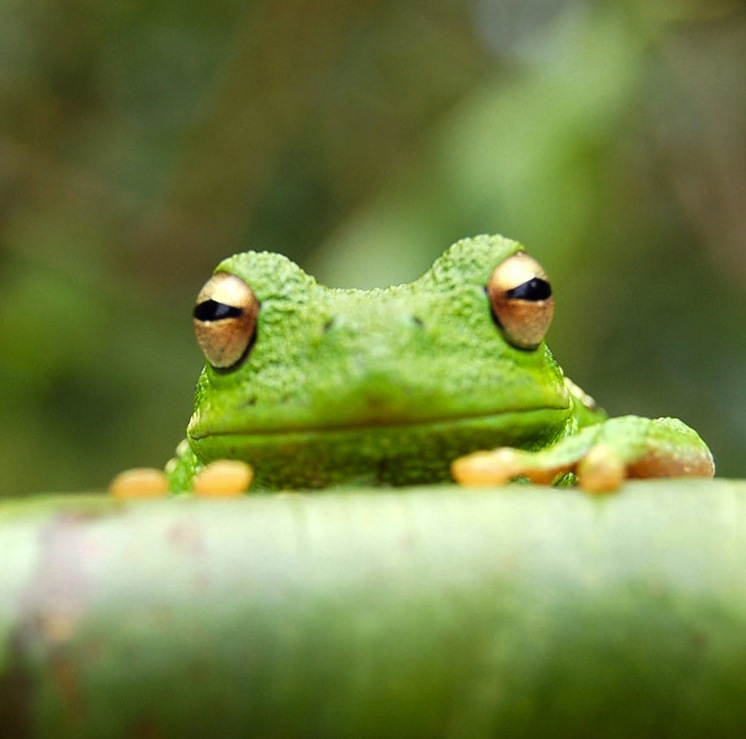
\includegraphics[width=2in]{frog.jpg}
    \end{columns}
    \vfill
    \begin{center}
    	You can also draw figures in \LaTeX{} using the PSTricks package.
    \end{center}
\end{frame}

%\begin{frame}{Making a poster using the beamerposter package.}
%	\begin{itemize}
%    	\item All commands are essentially the same to the \texttt{beamer} package
%    	\item Still working on the style file
%        \item Sections are broken out using the \texttt{block} command
%    \end{itemize}
%\end{frame}

%----------------------------------------------------- 
\begin{frame}[fragile]{BibTeX handles making the references and making the bibliography}
	\begin{columns}
    	\column{0.5\textwidth}
        	\begin{itemize}
            \item Just put your references (automatically generated by Google Scholar) in a .bib file that you reference at the end of the document, \cite{FineStructureConst,HallEffect}
            \item JabRef is also a powerful citation manager: \href{http://jabref.sourceforge.net/}{http://jabref.sourceforge.net/}
            \item You can also change the citation style: [Number], (Author,Year), etc. 
            \end{itemize}
        \column{0.5\textwidth}
            \centering
            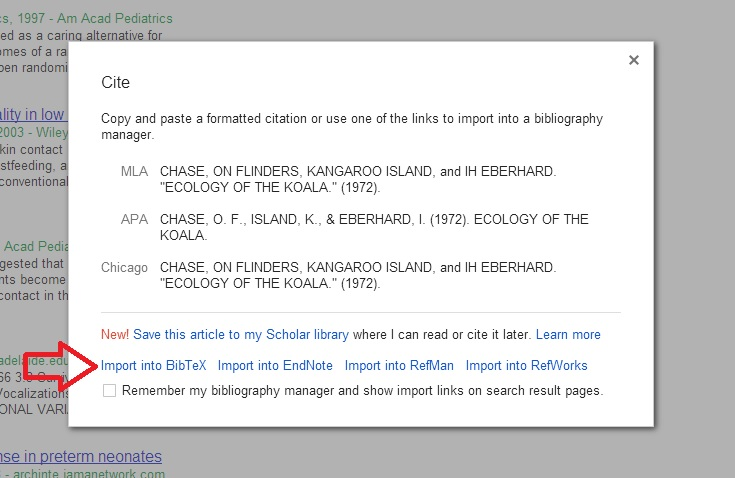
\includegraphics[width=2in]{ScholarPic.jpg}
    \end{columns}
	\vfill
	Just include \verb!\bibliographystyle{plain}! in the preamble and 	\verb!\bibliography{yourrefname.bib}! before the end of the doc.
\end{frame}

 %----------------------------------------------------- 
\begin{frame}{Quick prep: Markdown + \LaTeX{}}

	\begin{itemize}
    \item You can avoid formatting the documents and just get to the sweet, sweet math
    \item iPython and \href{stackedit.io}{stackedit.io} both have Markdown environments that can render \LaTeX{} using MathJax, a Javascript tool
    \item You can make quick presentations (in IPython), notes, handouts, etc.
    
    \end{itemize}

\end{frame}

 %----------------------------------------------------- 
\begin{frame}[allowframebreaks]{References}
	\bibliographystyle{unsrt}
	\bibliography{refs}
\end{frame}

\end{document}
